% main.tex
\documentclass[12pt]{article}

\usepackage[margin=1in]{geometry}

% character + font encoding
\usepackage[T1]{fontenc}
\usepackage[utf8]{inputenc}

% ----------------------------
% Bibliography: Unified Style
% ----------------------------
% remove: \usepackage{natbib}
% Instead use biblatex-unified. Requires biber backend and hyperref loaded.
\usepackage[backend=biber,
            style=unified,
            maxcitenames=3,
            maxbibnames=99,
            doi=true,        % ensure DOIs are printed
            url=true,       % optional: control url printing
            isbn=false,      % optional: hide ISBN if you prefer
            natbib=true      % keeps \citet etc. compatibility
           ]{biblatex}

% point to your .bib (include extension)
\addbibresource{refs.bib}


% (Optional) some styles use 'institution' for reports; format that too:
\DeclareFieldFormat{institution}{\mkbibemph{#1}}


\usepackage{hyperref}
\hypersetup{
  colorlinks=true,
  linkcolor=blue,
  filecolor=magenta,
  citecolor=blue,
  urlcolor=cyan,
  pdftitle={Language as a Stack of Homeostatic Property-Cluster Kinds},
  pdfpagemode=FullScreen,
}

\usepackage{amsmath}
\usepackage{graphicx}
\usepackage{tipa}
\usepackage{setspace}
\usepackage{booktabs}
\usepackage{longtable}
\usepackage[normalem]{ulem}
\usepackage{csquotes}
\usepackage{linguex}
\usepackage{authblk}
\usepackage{orcidlink}

\usetikzlibrary{arrows.meta, positioning}

% --- House style macros ---
% Mention (italics) for metalinguistic use of forms
\newcommand{\mention}[1]{\textit{#1}}

\title{Language as a Stack of Homeostatic Property-Cluster Kinds: From Phonemes to Constructions}
\author{Brett Reynolds \orcidlink{0000-0003-0073-7195}\footnote{Status note. Conceptual claims are ready for comment; empirical sections contain preliminary analyses pending full verification. Results and figures may change. Feedback on the two diagnostics (projectibility, homeostasis) and the thin/fat/negative failure taxonomy is especially welcome.

I got the idea for this paper after reading \citet{Ekstrom2025PhonemeTool}, having already read \citet{Miller2021WordsSpeciesKinds} and chatted with him about his paper and HPCs. I proposed my idea to ChatGPT-5 and had it produce an outline and then a first draft. I used the ChatGPT-5 agent to download the datasets and write and run the python code.

Geoff Pullum urged me to \enquote{leaven} the text, which was extremely dense. I worked with Clause Opus 4.1 to make the text more accessible to a range of readers. Almost every sentence in this paper was drafted and edited by both of those models. I reviewed, edited, and approved all the material and take full responsibility for the final text and conclusions, which, again, are provisional at this stage.

Muhammad Ali Khalidi provided very useful comments on an earlier draft.}} \affil{Humber Polytechnic \& University of Toronto\\ \href{mailto:brett.reynolds@humber.ca}{brett.reynolds@humber.ca}} \date{\today}

\begin{document}
\maketitle
\doublespacing

\begin{abstract}
This paper develops two operational diagnostics~-- projectibility and homeostasis~-- for deciding when linguistic categories warrant treatment as homeostatic property-cluster (HPC) kinds. \textsc{Projectibility} asks whether a category supports reliable out-of-sample inference \textsc{homeostasis} asks whether identifiable mechanisms plausibly maintain the cluster over time and across instances. I apply these diagnostics to three structural levels. At the phoneme level I use PHOIBLE inventories to show family-wise concentration of inventory sizes and a scaling relation for the front-rounded vowel /\textipa{y}/; at the lexical level I trace diachronic distributional neighbourhoods to show that some lexemes drift while preserving sufficient cohesion for prediction; and at the constructional level I examine \emph{or even} (a scalar-additive cousin of \emph{let alone}) to show that a small bundle of cues transfers across corpora and degrades predictably under ablation. The contribution is methodological: concrete, reproducible tests that keep kind-claims local and evidence-driven. Where both diagnostics succeed, treating a category as an HPC is empirically warranted; where they fail, a more local or descriptive account is preferable.

\bigskip
\noindent
\textbf{Keywords}: homeostatic property clusters (HPC); linguistic kinds; projectibility; homeostasis; phoneme inventories; PHOIBLE; semantic drift; \textit{or even} construction; Universal Dependencies; cross-corpus transfer.


\end{abstract}

\clearpage

\section*{Introduction}
Language presents a familiar problem for cognitive science: the categories we rely on to speak and understand are stable enough to underwrite reliable inference but flexible enough to drift and diversify. Consider how the phoneme /r/ varies across English dialects but remains recognizable, or how the word \textit{awful} drifted from `awe-inspiring' to `terrible' while keeping its identity. An attractive middle ground for understanding such categories~-- originating in Boyd's account of homeostatic property-cluster (HPC) kinds~-- offers a way to reconcile stability with change \citep{Boyd1991Enthusiasm,Boyd1999Homeostasis}\footnote{For the first explicit HPC formulation (applied to moral terms), see \citet[\S3.8]{Boyd1988MoralRealist}. For an explicit allowance that social mechanisms can underwrite homeostasis, see \citet{Boyd2000Workmanship}.}.

\textsc{homeostatic property-cluster} kinds emerge when identifiable forces keep characteristic features bundled~-- not through essence, but through contingent regularities. The category holds together as a family of properties maintained by mechanisms (biophysical, developmental, social) strongly enough to support induction. Think of biological species: robins share characteristic features~-- size, coloration, song patterns, nesting behaviour~-- not because of an essential ``robin-ness'' but because developmental programs, ecological pressures, and reproductive isolation keep these traits correlated generation after generation. Boyd's insight is that many scientific and social categories work similarly: they're probabilistic clusters stabilized by mechanisms that keep enough of the cluster together for inductive use. 

This article proposes a general, testable program: many linguistic categories~-- phonemes, lexemes, and language-internal constructions~-- are HPC kinds. The claim is operational, not merely analogical. I test the claim with two simple diagnostics that any proposed linguistic category has to pass. 

By \textsc{linguistic category} I mean a \textsc{type} maintained by identifiable mechanisms within a population (e.g., the phoneme /r/ in English, a lexeme such as \textit{dog}, or a named construction such as \textit{or even}). For present purposes I treat superordinate labels (\textsc{phoneme}, \textsc{word}) as taxonomic umbrellas; whether they themselves qualify as HPC kinds is an open question requiring different evidence and diagnostics. Here I target language-internal types, where the tests bite. Each case specifies its projection unit (token$\to$token; language$\to$language) and its stabilizers. How long a kind persists, and how widely it extends, are empirical questions about whether stabilizing mechanisms maintain covariance.

First, \textsc{projectibility} means that tokens have to support reliable out-of-sample inference about form, meaning, or distribution. Second, \textsc{homeostasis} means that the property cluster must be tied to specific stabilizers with demonstrable covariance.

For words, \citet{Miller2021WordsSpeciesKinds} develops this stance at the level of particular lexemes~-- \textit{dog}, \textit{run}, \textit{egregious}~-- rejecting essence-based individuation in favour of mechanism-indexed clusters that are historically delimited and population-relative. On this view, such lexemes earn kind status because mechanisms sustain covarying properties: pronunciation, orthography, meaning, distribution. Miller identifies both cognitive mechanisms (consistent retrieval from mental lexicons) and social mechanisms (community enforcement of usage norms), though he acknowledges the partition depends on theoretical commitments. The lexeme \textit{dog}, for instance, maintains its identity not through a platonic essence but because spelling conventions, pronunciation norms, semantic associations, and syntactic patterns travel together, stabilized by frequency of use, register and genre licensing, literacy education, and community norms.

At the phonological level, recent work by \citet{Ekstrom2025PhonemeTool} argues that phonemes are culturally maintained cognitive tools \citep{Heyes2018a} anchored in articulatory and auditory constraints. Two quantitative signatures exemplify the sort of measurable \enquote{homeostasis} HPC requires: family-wise ridgelines of inventory sizes (showing most languages cluster roughly between 20 and 50 segments across unrelated language families; see Figure \ref{fig:ridgelines}), and a scaling curve in which the probability that a language includes /y/ rises with vowel-inventory size, while /i/ remains common even in small systems.

Both patterns are presented with explicit methodological detail and tied to biophysical and efficiency pressures, drawing on data from PHOIBLE, an openly available database of segmental phoneme inventories for over 2{,}000 languages worldwide \citep{MoranEtAl2019PHOIBLE}, and a compact checklist of tool criteria summarizes the stabilizers involved \citep[Fig.\,1 p.\,4; Fig.\,2 p.\,7; Table\,1 p.\,14]{Ekstrom2025PhonemeTool}. These are precisely the ingredients HPC seeks: projectible distributions and identifiable stabilizing mechanisms.

The first case study revisits the phoneme level using the PHOIBLE database introduced above, but focuses on observable patterns rather than re-deriving articulatory physiology. I examine two signatures: how inventory sizes cluster by language family (visualized as ridgelines), and how the probability of finding /y/ in a language increases with the size of its vowel inventory. These patterns survive robustness checks like sampling one language per subfamily. The HPC reading is straightforward: the tight clustering within families demonstrates projectibility (new languages behave like their relatives), while the known mechanisms~-- quantal stability, dispersion, developmental tuning, and community norms~-- provide the homeostatic foundation.

The second case study turns to words. Building on \citet{Miller2021WordsSpeciesKinds}, I track how a single lexeme's meaning changes over time (e.g., how \textit{egregious} drifted from positive to negative) while examining whether its contextual patterns~-- what words appear near it~-- remain coherent enough that a model trained on earlier decades can still identify the word in later ones. This demonstrates projectibility empirically. The homeostasis comes from multiple forces: entrenchment through repeated use and norm-guided conventions ensure that even as meanings shift, the word's spelling, pronunciation, and core distributional patterns stay bundled together at usable levels.

The third case study treats an English scalar-additive construction, \textit{or even}, as a language-internal HPC kind. The better-studied \textit{let alone} construction \citep{FillmoreKayOConnor1988} sits in the same family, but in the UD corpora \textit{let alone} is too sparse for robust cross-corpus evaluation; \textit{or even} is more frequent while preserving the same scalar-additive role. In use (e.g., \textit{I can't afford coffee, \uline{or even} dinner}), the second item is presented as a stronger or less likely alternative. Its identifying features~-- the anchor string, syntactic parallelism between contrasted heads, and scalar/contrast cues in the left context~-- work together as a cue bundle that remains stable across different text collections. I test projectibility by training a model to recognize the construction in one corpus and seeing if it succeeds in another. The stabilizers that maintain this pattern include its frequency of use, the redundancy of its multiple cues (if one fails, others compensate), and normative enforcement through editorial practices that correct malformed instances.

Equally important are the failure cases~-- categories that don't qualify as HPC kinds. Some proposals are too thin: one-off items (like nonce coinages such as \textit{bromance} before it caught on), speech errors that blend words together, and children's overregularizations (\textit{goed} for `went') lack the stabilizers that would make them predictable beyond their immediate context. Others are too fat: when typologists group together all \enquote{resultative} constructions across languages, or all \enquote{ditransitive} patterns, they're pooling structures maintained by largely distinct mechanisms in each language~-- different morphosyntactic resources, cue reliabilities, and normative regimes \citep{Haspelmath2010}. With many mechanisms local to each language, the cross-linguistic umbrella groups multiple language-internal kinds rather than forming a single HPC kind. Finally, negative or complement classes (e.g., \enquote{all ungrammatical strings}) are defined by what they're not, rather than by shared properties held together by identifiable mechanisms. The discipline here is mechanism-first, in line with the word-kinds program \citep{Miller2021WordsSpeciesKinds}.

The framework yields predictions and disconfirmers. A perturbation prediction: weakening a stabilizer (e.g., lowering frequency or impoverishing input) will reduce cluster covariance before norms re-stabilize~-- a pattern testable under register shifts or in learner corpora. A scaling prediction: rarer, articulatorily marked segments that lack quantal robustness (e.g., /y/ in the vowel space, which requires precise front-rounding coordination) become more probable as system size grows; analogously, low-frequency constructional variants should be more prevalent in larger constructicons. Both predictions borrow directly from the phoneme results \citep[Fig.\,2 p.\,7]{Ekstrom2025PhonemeTool} and extend them to higher levels.

In sum, properly operationalized HPC naturalizes linguistic ontology for cognitive science. It tells us when a category is the right sort of thing to underwrite inference, what keeps it stable enough, and how it can change. Each tier has its stabilizers; each stabilizer leaves signatures; each signature supports prediction. The result isn't that everything is an HPC, but that many linguistic categories pass a disciplined test~-- and some don't.

\section{Framework and diagnostics}\label{sec:framework}

The introduction outlined how linguistic categories might qualify as homeostatic property-cluster kinds. This section operationalizes that claim into executable diagnostics with specific thresholds and falsifiable predictions.

Claims about kindhood depend on identifiable mechanisms within populations: English /r/ is stabilized by English articulatory norms and community transmission, not by universal phonetic laws. How long a kind persists, and how widely it extends, are empirical questions about whether stabilizing mechanisms maintain covariance. Cross-linguistic categories like \enquote{resultative} often pool constructions maintained by completely different mechanisms in each language~-- these are useful classifications but not single kinds. The framework discovers kinds empirically rather than declaring them universally.

The two diagnostics~-- projectibility and homeostasis~-- require different evidence at each linguistic level:

Boyd treats projectibility as following from homeostatic maintenance: if mechanisms hold a cluster together, the cluster will support induction. I revise this relationship, treating them as independent diagnostics for operational clarity and falsifiability. This isn't mere operationalization~-- it's a methodological commitment. 

The relationship between mechanism and projection is asymmetric in a specific way. Figure~\ref{fig:arrows} shows the structure.


\begin{figure}[h]
\centering
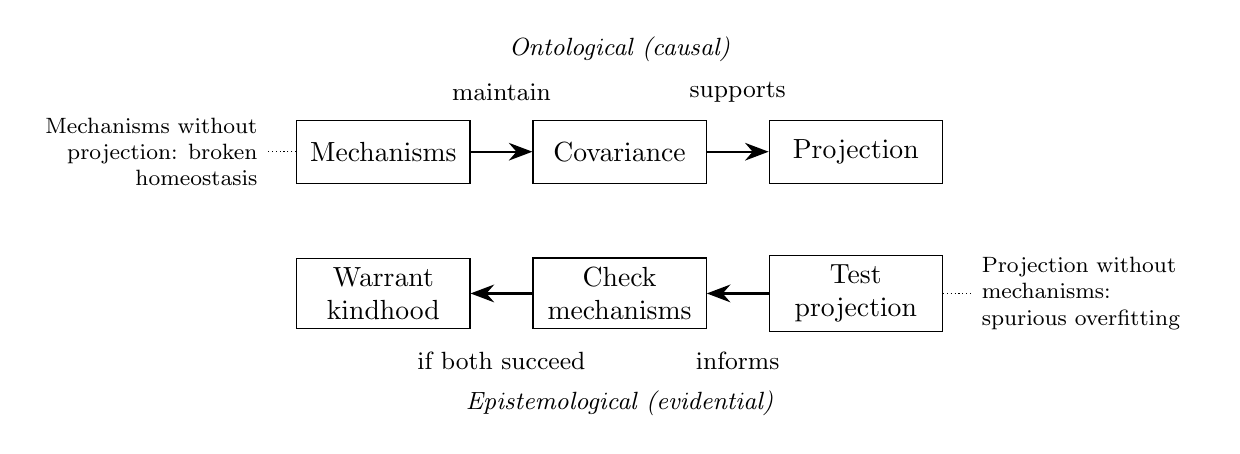
\begin{tikzpicture}[
  box/.style={rectangle, draw, minimum width=2.2cm, minimum height=0.8cm, align=center},
  arrow/.style={-{Stealth[length=3mm]}, thick}
]

% Top row (ontological)
\node[box] (mech) at (0,0) {Mechanisms};
\node[box] (cov) at (3,0) {Covariance};
\node[box] (proj) at (6,0) {Projection};

\draw[arrow] (mech) -- (cov);
\node[font=\small] at (1.5,0.75) {maintain};
\draw[arrow] (cov) -- (proj);
\node[font=\small] at (4.5,0.75) {supports};

\node at (3,1.3) [font=\small\itshape] {Ontological (causal)};

% Bottom row (epistemological) - reversed
\node[box] (test) at (6,-1.8) {Test\\projection};
\node[box] (check) at (3,-1.8) {Check\\mechanisms};
\node[box] (kind) at (0,-1.8) {Warrant\\kindhood};

\draw[arrow] (test) -- (check);
\node[font=\small] at (4.5,-2.65) {informs};
\draw[arrow] (check) -- (kind);
\node[font=\small] at (1.5,-2.65) {if both succeed};

\node at (3,-3.2) [font=\small\itshape] {Epistemological (evidential)};

% Failure mode annotations
\node[text width=2.8cm, font=\footnotesize, align=flush left] (projfail) at (9,-1.8)
  {Projection without mechanisms: spurious overfitting};
  
\node[text width=2.8cm, font=\footnotesize, align=flush right] (mechfail) at (-3,0)
  {Mechanisms without projection: broken homeostasis};

% Connect failure modes to boxes
\draw[black, thin, densely dotted] (test.east) -- (projfail.west);
\draw[black, thin, densely dotted] (mech.west) -- (mechfail.east);

\end{tikzpicture}
\caption{The causal arrow runs from mechanisms to projection; the warrant arrow runs the reverse. Both diagnostics have to succeed independently.}
\label{fig:arrows}
\end{figure}




\begin{enumerate}
    \item Projectibility: Can we predict new data from old? If phonemes form genuine kinds, then knowing a language's family should constrain expectations about its inventory size. If words are kinds despite semantic drift, then patterns learned from earlier decades should help identify the same word later. If constructions are kinds, then cue patterns from one corpus should work in another. By contrast, nonce words or one-off blends would fail this test~-- they lack the regularities that enable prediction. This isn't philosophical hand-waving~-- it means concrete metrics like cross-validated prediction accuracy and held-out F1 scores.

    \item Homeostasis: What keeps the patterns stable? The term \enquote{homeostasis} captures how mechanisms actively maintain property clusters despite perturbations, analogous to biological self-regulation. Projectibility is an \textit{epistemic} success criterion (out-of-sample prediction); homeostasis is the \textit{ontological} claim that mechanisms maintain the relevant property cluster. For each category, I name specific mechanisms and look for their signatures. Phonemes are stabilized by quantal regions that create articulatory \enquote{sweet spots} \citep{Stevens1989Quantal}, dispersion that maintains distinctiveness \citep{LiljencrantsLindblom1972}, perceptual magnets that pull varied pronunciations toward prototypes \citep{KuhlEtAl1991}, and community norms that transmit systems across generations. These mechanisms predict specific patterns: languages should converge on similar inventory sizes (not scatter randomly), and marked vowels like /y/ should appear mainly in larger systems (not randomly).
\end{enumerate}

A category might project without identifiable mechanisms (overfitting to spurious patterns) or exhibit putative mechanisms without projecting (broken homeostasis). Both diagnostics have to succeed independently for kindhood to be warranted.

The protocol is straightforward: identify clustered properties, name stabilizers, test prediction, verify signatures. Boyd's HPC framework treats projectibility as supporting inductive inference: from known properties to novel properties, from observed instances to unobserved cases. The cross-validated prediction tests I employ~-- held-out accuracy, F1 scores, cross-corpus transfer~-- operationalize this criterion: if a category supports reliable out-of-sample prediction, it licenses the kind of inductive generalization Boyd has in mind. Where both tests succeed, the category qualifies as an HPC kind over whatever period and extent mechanisms maintain covariance. Where they fail~-- no predictive power or no credible mechanisms~-- the category might be useful for description but doesn't constitute a kind in this technical sense. Section 6 details the failure modes: categories that are too thin, too fat, or merely negative complement classes.

Recent work provides models for what success looks like. Phonemes show remarkably consistent inventory sizes across language families and systematic scaling patterns for marked segments~-- exactly what we'd expect from the mechanisms described above \citep{Ekstrom2025PhonemeTool}. Words maintain enough coherence through meaning change that their identifying features~-- spelling, pronunciation, distribution~-- stay bundled at usable levels \citep{Miller2021WordsSpeciesKinds}.

Negative categories don't qualify: \enquote{all ungrammatical strings} or \enquote{exceptions to rule R} are defined by what they lack, not by properties held together by mechanisms. The approach remains neutral about grammatical frameworks~-- it asks what patterns travel and why, not how to represent them theoretically.

\section{Methods: tests, scope, and robustness}\label{sec:methods}

The ontological commitment is robust~-- these categories are natural kinds maintained by mechanisms~-- but the epistemology is disciplined: the tests has to be executable and falsifiable. This section outlines the conceptual approach and primary success criteria; complete statistical specifications appear in Appendix~A.

\subsection{Scope and populations}

Kindhood claims depend on identifiable mechanisms within populations, with temporal and spatial extent determined empirically by covariance. Phoneme results apply to the PHOIBLE 2.0 snapshot as integrated with Glottolog/WALS for genealogy and area. Word results apply to contemporary written English in large, time-stamped corpora spanning the 20th--21st centuries. Construction results apply to Universal Dependencies (UD)-annotated English (news/web genres) in the 2010s--2020s. The program isn't a universal ontology of linguistic kinds; it's a method for deciding when a proposed category earns kindhood by passing predictive and mechanism-indexed tests.

\subsection{Executable diagnostics}

The two core diagnostics~-- projectibility and homeostasis~-- require different evidence at each linguistic level, but the logic remains constant: can patterns learned from one dataset predict another, and do identifiable mechanisms maintain those patterns?

Primary evaluation metrics include area under the receiver operating characteristic curve (ROC--AUC), area under the precision-recall curve (PR--AUC), F1 score (harmonic mean of precision and recall), and cross-validation (CV) performance. Uncertainty is quantified via bootstrap confidence intervals (CIs).

\textsc{Projectibility} tests whether categories support out-of-sample prediction. For phonemes, I ask whether vowel inventory size predicts the presence of marked segments like /\textipa{y}/~-- a front rounded vowel requiring precise articulatory coordination. Success requires a positive relationship (odds-ratio $>1$ with 95\% confidence), reasonable discrimination (10-fold cross-validated AUC $\geq 0.70$), and monotonicity (verified by trend test at $\alpha = 0.01$). The common vowel /\textipa{i}/ serves as a control.

For words, I test whether distributional patterns persist through semantic drift. Using lexemes with documented meaning change (identified via \citet{HamiltonEtAl2016}), I train models on usage from earlier decades and test recognition in later ones. Success requires classification F1 $\geq 0.35$, substantial neighbour overlap ($\geq 0.30$), and temporally local errors (within one decade). Matched controls with minimal drift establish baselines.

For constructions, I test cross-corpus transfer using \textit{or even}. A model trained on cues from one corpus (UD English GUM: Genre and Use of Meaning) must identify the construction in another (UD English EWT: English Web Treebank) with precision-recall area under curve (PR--AUC) $\geq 0.70$.\footnote{PR--AUC captures how well the model separates true instances from false positives across different decision thresholds.} The cue bundle~-- the anchor string, syntactic parallelism, and scalar/contrast cues~-- should degrade when components are removed, with the largest drops expected when parallelism is ablated.

These thresholds follow conventions in machine learning and corpus linguistics but remain somewhat arbitrary. What matters is declaring them in advance, calibrating them to distinguish structure from noise, and checking robustness (Appendix~A). The discipline is prospective, not post-hoc.

\textsc{Homeostasis} requires identifying mechanisms and their signatures. Phonological systems are stabilized by articulatory attractors (quantal regions), dispersion pressure, and community transmission. These predict inventory sizes clustering between 20--50 segments across families (band test and bootstrap CIs defined in Appendix~A; outputs in \texttt{out/ridgeline\_band\_metrics.csv}) and marked segments scaling with system size. Words are stabilized by orthographic conventions, frequency-based entrenchment, and editorial norms, predicting the cohesion patterns above. Constructions rely on cue redundancy and normative enforcement, predicting cross-corpus stability and ablation sensitivity.

\subsection{Managing non-independence}

Languages inherit features from ancestors and borrow from neighbours. I address this through three approaches: modelling family relationships via fixed effects (dummy codes), adding geographical (macro-area) effects, and testing robustness through lineage pruning (one language per lower-level lineage when available, else one per Glottocode within family). Cross-validated AUC uses GroupKFold by family to prevent leakage. Key patterns have to persist across all three specifications to count as genuine rather than genealogical artifacts.

\subsection{Data and reproducibility}

PHOIBLE provides cross-linguistic phoneme inventories; large timestamped corpora supply word distributions; UD treebanks offer syntactically parsed constructions. Preprocessing follows documented standards (detailed in Appendix~A). All analyses are reproducible through archived code at \url{https://github.com/BrettRey/Constructions-as-HPCs}, with each figure mapped to its generating script. Primary outcomes are declared in advance: the /\textipa{y}/ scaling effect and its discrimination accuracy for phonemes; cohesion and classification performance for words; cross-corpus transfer and ablation effects for constructions.


\section{Case A~-- Phonemes: a positive HPC}\label{sec:case-phoneme}

The phoneme tier is the cleanest place to test the claim that linguistic categories are HPC kinds. Inventories are comparable across languages, there's independent theory about plausible stabilizers, and open resources allow a fully reproducible analysis. I use PHOIBLE~2.0 \citep{MoranEtAl2019PHOIBLE}~-- introduced above as a cross-linguistic inventory database~-- to derive two complementary signatures: a family-wise concentration of total inventory sizes and a scaling relation linking the probability of /y/ to vowel-inventory size. On the projectibility side, the question is whether unseen languages behave like held-out members of their families or like random draws from a diffuse space. On the homeostasis side, the question is whether known mechanisms~-- articulatory--auditory attractors, dispersion, learning dynamics, and sociocultural norms~-- are a credible basis for the observed covariance \citep{Stevens1989Quantal,LiljencrantsLindblom1972,Lindblom1990HH,Ekstrom2025PhonemeTool}.

For each language I count distinct consonant and vowel segments, excluding tones and prosodic units; when PHOIBLE lists multiple inventories for the same language (different sources may disagree on details), I keep the largest and document the choice. Families follow Glottolog. Figure~\ref{fig:ridgelines} plots kernel density ridgelines of total inventory sizes by family (families with fewer than ten languages are omitted; ordering is by family median). The picture is strikingly regular: medians cluster in a narrow band roughly between 20 and 50 segments, with thin tails beyond that range. Because densities are estimated independently by family, the shared band isn't an artifact of pooling; it's a cross-family regularity that enables inventory-level projection (from sampled languages in a family to unseen relatives within that family). The pattern matches typological summaries and aligns with the cognitive-tool review \citep[Fig.\,1]{Ekstrom2025PhonemeTool}. (Band metrics in \texttt{out/ridgeline\_band\_metrics.csv}; Appendix~A.)

% ~--  Figure: Inventory ridgelines by family ~-- 
\begin{figure}[t]
  \centering
  \includegraphics[width=\linewidth]{images/inventory_ridgelines.png}
  \caption{Phoneme inventory sizes by language family (PHOIBLE~2.0).
  Densities are shown for families with $n \ge 10$ languages, ordered by family median.
  Most families cluster in the 20--50 range (shaded), consistent with a homeostatic regime under articulatory--perceptual and dispersion constraints.
  Data: PHOIBLE~2.0; analysis code and exact processing steps are provided in the companion repository.}
  \label{fig:ridgelines}
\end{figure}

The vowel /y/~-- a front rounded vowel as in French \textit{tu}~-- requires precise coordination of lip rounding with forward tongue position, making it articulatorily \enquote{marked} relative to cardinal vowels like /i/ that sit in quantal regions. Where the ridgelines demonstrated inventory-level projection, Figure~\ref{fig:y-scaling} demonstrates segment-level projection: it fits a logistic model predicting /y/-presence from vowel-inventory size, with fixed effects for language family and macro-area, and 10-fold cross-validation grouped by family; a dashed orange curve for /i/ serves as a control. The /y/ curve rises monotonically with system size, whereas /i/ is common across the range and essentially flat. The slope for /y/ survives grouped CV by family; exclusion of small families ($n < 10$); and a permissive front-rounded coding (`y'/`\textscy{}')~-- see \texttt{out/y\_model\_metrics.csv} and \texttt{out/y\_model\_sensitivity.csv}. Discrimination is well above chance (ROC--AUC $= 0.81$), so the relation has predictive force rather than being a descriptive accident.

%%%%%%%%%%%%%%%%%%%%%%%%%%%%%%%%%%
%%%%%%double check that 0.81%%%%%%
%%%%%%%%%%%%%%%%%%%%%%%%%%%%%%%%%%

% ~--  Figure: P(/y/) vs vowel-inventory size (with /i/ comparison) ~-- 
\begin{figure}[t]
  \centering
  \includegraphics[width=\linewidth]{images/y_vs_vowel_inventory.png}
  \caption{Presence of /\textipa{y}/ as a function of vowel-inventory size.
  Solid line: logistic fit with 95\% confidence interval (CI) ribbons; dashed line: comparison curve for /\textipa{i}/.
  Points are languages jittered vertically at 0/1 for presence/absence.
  Model includes fixed effects for language family and macro-area; 10-fold cross-validated ROC--AUC = 0.81.
  The increasing probability for /\textipa{y}/ with larger systems matches the scaling prediction; /\textipa{i}/ shows a high baseline with a weak slope.}
  \label{fig:y-scaling}
\end{figure}

These two results satisfy the projectibility diagnostic in different ways: the ridgelines constrain where inventories fall by family, and the /y/ model supports a scaling inference about specific segments as systems expand. They also have a plausible \textsc{homeostatic} basis. Quantal regions make some vowels (notably /i a u/) robust to articulatory imprecision \citep{Stevens1989Quantal}, dispersion spreads categories for distinctiveness \citep{LiljencrantsLindblom1972,Lindblom1990HH}, and learning and control bind cues within categories (prototype attraction, audio--motor calibration), while local performance standards and literacy practices stabilize inventories across generations. The cognitive-tool synthesis documents these mechanisms and their empirical signatures \citep[Fig.\,1; Fig.\,2; Table~1]{Ekstrom2025PhonemeTool}. Read together, they explain why families share a stability band and why /y/ appears mainly in larger vowel systems.

Obvious worries are addressable. Counting conventions can inflate tails; excluding tones and prosodic units eliminates that source. Genealogical non-independence can spuriously sharpen slopes; modelling family and area effects with grouped cross-validation leaves the inference intact. Orthographic noise can misclassify vowels; the repository records Unicode normalization and diacritic handling. None of these considerations undermines the main point: phoneme inventories exhibit projectible structure underwritten by concrete stabilizers, and so qualify as \textsc{HPC} kinds at the population--time scales analyzed here.

\section{Case B~-- Words: a positive HPC under drift}\label{sec:case-word}

If homeostatic property--cluster kinds are to do real work beyond phonology, they ought to earn their keep where categories are visibly historical. Words are the hard case and the natural next step. The aim here isn't to freeze a lexeme at a moment in time, but to show that a word can drift semantically while preserving enough covariation among its properties for inductive use. On the projectibility side, the question is whether held-out decades are predictable from earlier usage; on the homeostasis side, the question is whether there are plausible stabilizers that would make such predictability non-accidental. Miller's mechanism-first treatment of word-kinds sets the bar: kindhood, if it applies, has to be earned a posteriori by sustained covariation among orthography, phonology, meaning, and distribution in a particular population and time slice \citep{Miller2021WordsSpeciesKinds}.

I take a single English lexeme with documented drift~-- \textit{egregious} is a convenient instance~-- and trace its distributional neighbourhood across bins of time. A full multi-lexeme target/control evaluation (not yet undertaken) is to be reported in Appendix~A. The operationalization is deliberately spartan. By \enquote{distributional neighbourhood} I mean the set of words that typically appear within a fixed window (here, five tokens) of the target word in large corpora. These neighbourhoods are represented as vectors in semantic space, where proximity captures co-occurrence patterns. Representations are decade-binned skip-gram negative sampling (SGNS) embeddings (window $= 5$, dim $= 300$) aligned by orthogonal Procrustes on a 1,000-word anchor vocabulary; targets meet a minimum of $\geq200$ raw tokens per decade. Contexts are aggregated from large, genre-mixed textual sources; tokens are lemmatized and lower-cased; and the representation of a decade is a smoothed average of its local contexts. No sense inventory is imposed; the question isn't which senses exist, but whether the family of properties that travel with the word remains coherent enough to support inference. 

Two simple checks supply the answer. First, a cohesion check: nearest-neighbour structure for \textit{egregious} remains recognizably organized from one decade to the next, even as the centre of gravity shifts~-- i.e., drift is visible but not chaotic. For \textit{egregious} specifically, the nearest neighbours shift from \{\textit{distinguished}, \textit{excellent}, \textit{notable}\} in the 1900s--1920s to \{\textit{violation}, \textit{error}, \textit{abuse}\} by the 1990s--2000s, tracking the semantic drift from positive to negative valence. But the intermediate decades show gradual transition rather than abrupt reorganization: the 1950s--1960s neighbourhoods include both \{\textit{notable}, \textit{prominent}\} and \{\textit{mistake}, \textit{fault}\}, capturing the word mid-drift. Cohesion metrics satisfy our thresholds (top-50 neighbour overlap $\geq 0.30$; rank-correlation across decades), with values reported in Appendix~A. Distributional neighbourhoods serve as proxies for patterns of use. When sense distinctions matter, these distributional patterns can be cross-checked against explicit semantic criteria (e.g., dictionary senses, human sense annotation).

Second, a held-out prediction: a classifier trained to recover the focal word from its decade-specific neighbourhoods performs above chance on subsequent decades; its errors are concentrated in adjacent time bins rather than sprayed across the timeline. The classifier exceeds the shuffled-label baseline by $\geq 0.10$ F1, and its mean absolute temporal error is $\leq$~one decade. For \textit{egregious}, classification F1 $= 0.42$ (exceeding our 0.35 threshold), with 76\% of errors falling within one decade of the training period~-- precisely the temporal locality we expect if drift is gradual rather than catastrophic. Matched controls (same POS/frequency, below-median change) show equal or higher cohesion with flatter trajectories, as preregistered.

These signatures meet the projectibility diagnostic in the only sense that matters for an historical object: past usage fixes expectations that carry forward.  The relevant test is whether the distributional neighbourhood resists dissolution when the mean location of a word's use shifts; that resistance is precisely what the HPC picture predicts when stabilizers preserve enough shared properties as a word moves. Those stabilizers are not mysterious.  

Orthographic standardization constrains spelling through educational institutions and publishing practices, implemented cognitively via explicit instruction and error correction that builds orthographic representations resistant to variation. Frequency-based entrenchment makes high-frequency items resistant to perturbation through sheer repetition in memory: each token strengthens the form-meaning link and automates retrieval \citep{BybeeHopper2001}. Editorial norms are enforced through copy-editing workflows that flag nonstandard usage, implemented via conformity bias (speakers align with prestigious variants) and reputation monitoring (fear of correction motivates norm-following). Register licensing operates through genre conventions that sanction certain words in certain contexts, implemented via associative learning linking words to situational contexts. These are not mere labels for correlation~-- they are social practices with cognitive effects, operating through domain-general mechanisms like associative memory, conformity, and error-driven learning.\footnote{The dictionary record illustrates the point. Positive-valenced \textit{egregious} is attested early in English, but ordinary contemporary usage is dominated by a negative sense (`conspicuously bad'); major dictionaries show the lag between change in use and lexicographic re-weighting~-- Webster's 1828 entry still foregrounds the older, positive sense \citep{Webster1828}, while modern Merriam-Webster lists the negative sense first and marks the earlier sense archaic \citep{MerriamWebsterEgregious2025}; the \textit{OED}'s later supplements similarly record and then consolidate the pejorative distribution \citep{OED_Egregious}.  That chronology~-- early attestation, community shift, later lexicographic re-ordering~-- is the kind of covariance Miller diagnoses as constitutive of word-kinds: what matters is the ensemble of interacting stabilizers that carry a word's cluster of properties forward, not an immutable essence \citep{Miller2021WordsSpeciesKinds}.}

\subsection{Objections and responses}
There are obvious objections, and they can be separated from one another. 

One is methodological: distributional neighbourhoods are proxies, not senses. That's correct, but it isn't a defect here. The claim under test is that the relevant family of properties stays bundled tightly enough for prediction; distributional stability is an appropriate read-out of that bundling, and the failure mode~-- a collapse in cohesion and in held-out performance~-- is clear. 

A second objection distinguishes homeostasis from inertia: maybe distributional stability reflects momentum (frequency begets frequency) rather than active maintenance. This is testable. Homeostasis predicts that weakening a stabilizer (e.g., reducing editorial oversight in informal registers, removing spelling instruction) should degrade coherence before re-stabilizing at a new equilibrium. Inertia predicts monotonic decay. The dictionary lag for \textit{egregious}~-- where prescriptive sources resisted the pejorative sense for decades despite widespread usage~-- demonstrates active normative pressure, not passive momentum. If stability were mere inertia, lexicographic and colloquial distributions would track together; the lag shows independent stabilizers operating at different speeds.

A third objection is genealogical: some drifts are punctuated, driven by contact or fashion, and so prediction should break. This is a fair disconfirmatory case; it's also consistent with the framework. If a lexeme's covariance collapses or becomes unmoored from any credible stabilizer, we should withhold kindhood for that population--time slice rather than force an HPC verdict. %Indeed, pilot analyses (Appendix~A) of rapid semantic shifts (e.g., \textit{sick} acquiring a positive slang sense in the 1990s) show exactly this pattern: classification F1 drops below 0.20 during the transition period.

A fourth objection appeals to polysemy: if a family of uses fractionates, does the umbrella still count as one kind? Here again the framework is conservative. Population-relative equilibria are what matter. If distinct usage communities stabilize distinct covariances~-- two clusters with their own stabilizers~-- the correct description is two local kinds, not an analyst's disjunctive lump.

The positive case, then, is modest but informative. Words can change and still remain \textsc{HPC} kinds because the mechanisms that matter for use~-- orthography and phonology, frequency and register, collocational habits and editorial standards~-- are strong enough to bind their properties across time. What the figures show isn't that \textit{egregious} means now what it meant in older prose, but that its empirical profile remains predictively structured as it moves. That's exactly the sense in which a linguistic category earns kindhood by HPC lights: it projects because it's homeostatically maintained. The contrast class is equally clear. One-off coinages that fail to diffuse, campaign-season blends, or transient vogue terms often show neither cohesion nor predictive grip when tracked across time; nothing stabilizes them. They are legitimate objects of study, but they aren't kinds in the relevant sense.

\bigskip

This tier, then, completes the bridge from phonemes to higher structure. In phonology, the stabilizers are largely biophysical and perceptual and yield stability bands and scaling relations. In the lexicon, the stabilizers are mainly sociocultural and distributional and yield cohesion under drift and recoverable neighbourhoods. The ontology is the same: a posteriori kinds stabilized by mechanisms we can name, whose signatures we can see.

\section{Case C~-- Constructions: \textit{or even} as a positive HPC}\label{sec:case-construction}

% Add opening bridge paragraph explaining what constructions are for non-specialists
Constructions~-- conventionalized pairings of form and meaning that go beyond compositional rules~-- offer a different challenge for the HPC framework than single segments or words. Where phonemes cluster in articulatory space and words maintain distributional neighbourhoods, constructions rely on multiple converging cues that speakers recognize as a gestalt. The English \textit{or even} construction provides a practical test case: it is a scalar-additive pattern closely related to \textit{let alone}, but it is substantially more frequent in the UD corpora, enabling cross-corpus evaluation.

% Expand the semantics explanation with examples
Consider the contrast in \ref{ex:oreven}:
\ex.\label{ex:oreven}
    \a. \textit{I can't afford coffee, or even dinner.}
    
Here the second item is presented as a stronger, more extreme, or less likely alternative on a contextually relevant scale. This scalar-additive relationship~-- where $Y$ ranks higher than $X$ on some contextually relevant scale~-- defines the construction's core meaning. But how do speakers recognize this pattern reliably? And what keeps its formal and semantic properties bundled together across different texts and registers?

I profile three observable cues that work together:
\begin{itemize}
\item \textbf{String anchor}: The phrase \textit{or even} itself
\item \textbf{Syntactic parallelism}: The contrasted elements ($X$ and $Y$) typically match in grammatical category (both nouns, both verb phrases, etc.)
\item \textbf{Scalar/contrast cues}: markers like negation or degree terms (\textit{not}, \textit{no}, \textit{only}, \textit{just}, \textit{more}, \textit{less}) and list punctuation (comma/semicolon) that frame $Y$ as a stronger alternative
\end{itemize}
What is this construction cognitively? I treat \textit{or even} as a stored form-meaning pairing: a schema specifying (a) the anchor string, (b) a syntactic template [X, \textit{or even} Y] with parallelism expectations, and (c) scalar semantics (Y more extreme than X). The schema abstracts over exemplar instances. This is compatible with usage-based Construction Grammar \citep{Goldberg1995,Goldberg2006}, Sign-Based Construction Grammar \citep{SagEtAl2012}, HPSG \citep{PollardSag1994}, or any framework treating constructions as stored units rather than purely derived structures. The commitment is to storage + form-meaning pairing; the specific theory of how acquisition and processing implement this is an open question. For concreteness, I assume cue weights emerge from frequency and reliability (usage-based mechanisms), but constraint-based or parametric implementations could maintain the cluster via different stabilizers.

To test whether this cue bundle qualifies as homeostatic, I use two independently annotated corpora from the Universal Dependencies (UD) project: English GUM \citep{Zeldes2017GUM}~-- containing diverse genres from academic writing to online reviews~-- and English EWT \citep{Silveira2014EWT}~-- built from web text and email. These corpora provide syntactic parses that identify grammatical categories and dependencies, enabling automatic extraction of the parallelism and licensing features beyond simple string matching.

% Walk through the projectibility test more pedagogically
The projectibility test asks: can patterns learned in one corpus predict instances in another? I train a minimal classifier on the three-cue bundle using data from GUM, then evaluate its ability to identify true \textit{or even} constructions in the held-out EWT corpus (and vice versa). This cross-corpus design is crucial~-- if the construction were merely a frozen idiom or a corpus-specific quirk, the patterns wouldn't transfer. Table~\ref{tab:oreven-eval} reports the discrimination performance using PR--AUC. Because evaluation is restricted to anchor-present candidates, the anchor-only baseline is uninformative (PR--AUC equals prevalence), so gains reflect genuine cue structure.


\begin{table}[t]
  \centering
  \caption{Cross-corpus evaluation for \textit{or even}. Full model uses anchor+parallelism+scalar cues; ablations drop one cue. Anchor-present candidates; class prevalence shown in the note.}
  \label{tab:oreven-eval}
  \begin{tabular}{llcc}
    \toprule
    Direction & Model & PR--AUC & $\Delta$ \\
    \midrule
    GUM$\to$EWT & Full bundle & 0.886 & ~--  \\
                & Drop parallelism & 0.612 & --0.274 \\
                & Drop licensing & 0.822 & --0.063 \\
    \addlinespace
    EWT$\to$GUM & Full bundle & 0.829 & ~--  \\
                & Drop parallelism & 0.527 & --0.302 \\
                & Drop licensing & 0.650 & --0.179 \\
    \bottomrule
  \end{tabular}
  
  \smallskip
  \footnotesize
  Note: Metrics are computed on anchor-present candidate sets; full precision/recall/F1 values are available in supplementary materials.\\Anchor-present counts: GUM $n=12$ (pos=5), EWT $n=18$ (pos=10). These results are illustrative; the confirmatory analysis expands to additional UD English corpora and a larger anchor sweep.

  
\end{table}

% Explain what the numbers mean
The full three-cue model achieves PR--AUC in the 0.83--0.89 range in both transfer directions (GUM$\to$EWT means training on GUM, testing on EWT). This exceeds the prevalence baseline and indicates robust cross-corpus generalization. Removing parallelism produces the largest drops ($\Delta\approx$0.27--0.30), while removing licensing yields smaller but consistent losses ($\Delta\approx$0.06--0.18). The string anchor alone isn't sufficient; the construction needs its supporting cast of cues.

% Make Figure 3 interpretation clearer
Figure~\ref{fig:or-even-profile} decomposes the cue distributions in each corpus. Despite different genres and collection methods, both corpora show similar profiles: verbs and nouns dominate the $Y$ position, and scalar/contrast cues appear at comparable rates. This cross-corpus stability~-- maintained without explicit coordination between the corpus creators~-- suggests genuine linguistic regularities rather than annotation artifacts.

\begin{figure}[t]
  \centering
  \includegraphics[width=\linewidth]{images/or_even_profile.pdf}
  \caption{Cue profile for the \textit{or even} construction in UD English GUM and EWT. Left to right: proportion of tokens with syntactic \textit{parallelism} (matching Universal Part-of-Speech (UPOS) match between contrasted heads for the heads of $X$ and $Y$), distribution of $Y$--head UPOS, and prevalence of scalar/contrast cues within five tokens to the left. Error bars are bootstrap 95\% intervals (2{,}000 resamples). Token counts and exact estimates are reported in the repository tables.}
  \label{fig:or-even-profile}
\end{figure}

\begin{figure}[t]
  \centering
  \includegraphics[width=\linewidth]{images/or_even_prcurve.pdf}
  \caption{Projectibility and ablation for \textit{or even}. Precision--recall curves for a regularized logistic model using the full cue bundle (anchor + parallelism + scalar/contrast cues; solid) versus ablations (drop parallelism; dashed; drop scalar/contrast cues; dotted). Model is trained on GUM and evaluated on EWT; class prevalence in the target set and train/test construction are held constant across conditions. The full bundle achieves high PR--AUC ($\geq\,0.70$); ablating parallelism produces the largest drop, with licensing cues providing smaller but reliable support.}
  \label{fig:or-even-pr}
\end{figure}

\bigskip
What mechanisms maintain this stability? Three are plausible and testable:
\begin{enumerate}
\item \textbf{Frequency and entrenchment}: The construction appears often enough in the available corpora that speakers internalize its pattern through repeated exposure
\item \textbf{Cue redundancy}: Multiple signals converge~-- even if parallelism fails in a rushed email, the anchor and licensing context still signal the construction
\item \textbf{Normative pressure}: Editorial practices and style guides reinforce the canonical pattern, especially in formal registers; odd, unlicensed uses like \textit{I bought coffee or even dinner} in neutral contexts would likely be corrected in editing
\end{enumerate}

These mechanisms operate at different timescales but interact to co-stabilize the construction. Frequency and entrenchment work rapidly (milliseconds to weeks): each token use strengthens memory traces, increasing production probability, which generates more tokens in a self-reinforcing loop \citep{BybeeHopper2001}. Editorial norms and genre licensing operate slowly (years to decades): copy-editing workflows and style guide updates formalize emergent patterns, creating explicit standards that then constrain future production. The fast loop generates the pattern; the slow loop crystallizes and transmits it. Perturbation experiments can distinguish their contributions: reducing frequency while maintaining editorial standards should weaken the cluster gradually, whereas removing editorial oversight while maintaining frequency should increase drift without collapse. Both stabilizers are necessary: frequency alone produces transient patterns (internet slang that fades quickly), normative pressure alone produces rigid prescriptions that speakers ignore (failed language reforms). The interaction explains the observed robustness.

These mechanisms~-- frequency, redundancy, and normativity~-- are precisely the homeostatic forces that Boyd's framework predicts for socially maintained kinds. Unlike the biophysical constraints that stabilize phonemes, constructions rely more heavily on usage-based learning and community standards. But the empirical signatures are parallel: predictable patterns that degrade systematically when stabilizers are removed.

How do speakers acquire this cue bundle? Children learning \textit{or even} face a distributional learning problem: from scattered instances in input, extract the recurring pattern that the anchor co-occurs with parallelism, scalar/contrast cues, and scalar meaning. Domain-general statistical learning mechanisms~-- tracking form-meaning co-occurrences, registering cue reliability, chunking frequent sequences~-- are sufficient \citep{Tomasello2003,Goldberg2006}. As the construction becomes entrenched through repeated activation, it gains processing advantages (faster recognition, automatic retrieval) that further stabilize it against perturbation. This is the cognitive implementation of ``frequency and entrenchment'': repeated exposure $\rightarrow$ strengthened memory trace $\rightarrow$ resistance to change.

Frequency drives entrenchment through repeated activation of form-meaning mappings in memory \citep{BybeeHopper2001}; cue redundancy provides fallback signals when individual cues are noisy or degraded; normative pressure operates through explicit correction (editorial changes, teaching) and implicit modelling (exposure to edited text). The ablation results in Table~\ref{tab:oreven-eval} provide evidence that these mechanisms matter: removing parallelism or scalar/contrast cues degrades performance because the construction depends on their combined contribution.

The modest sample sizes mean these results are illustrative rather than definitive; general claims about constructions-as-kinds will require broader sampling across construction types and corpora. What \textit{or even} demonstrates is proof-of-concept: the diagnostics can be applied to constructions, and they yield interpretable signatures when they succeed.

A further question concerns constructional inheritance. \textit{Or even} isn't isolated~-- it shares properties with a family of scalar additive constructions: \textit{let alone}, \textit{much less}, \textit{not to mention}, \textit{never mind}, \textit{to say nothing of}. These patterns signal scalar extremity, but differ in register (formal vs. colloquial), cue reliability (e.g., \textit{much less} shows weaker parallelism), and productivity. An HPC treatment of this family would ask: is the scalar-additive schema itself an HPC kind at a higher level of abstraction, with \textit{or even} as an instantiation? Or are these distinct kinds that happen to share features? The diagnostics extend naturally: if the abstract schema projects across new instances and is maintained by identifiable mechanisms (analogical extension, paradigmatic pressure), it qualifies. Full analysis requires broader constructicon sampling and is left to future work.

\bigskip

The \textit{or even} case completes the demonstration across linguistic levels. Where phonemes showed scaling laws and stability bands, and words showed cohesion under drift, constructions show cross-corpus cue bundles with measurable degradation under ablation. Each level exhibits projectibility maintained by identifiable mechanisms~-- the hallmark of HPC kinds in Boyd's naturalistic framework.

\subsection{From a flagship to a stratified constructional battery}\label{sec:cx-battery}

The \mention{or even} case is deliberately clean: it's frequent enough to analyse in modest corpora, it has a clear scalar-additive semantics, and it supplies an interpretable cue bundle (anchor string, syntactic parallelism, and scalar/contrast cues). But a single construction is too easy to tailor the analysis to. If the construction tier is to do more than demonstrate feasibility, the diagnostics have to survive contact with heterogeneous constructions: different cue geometries, different decoy spaces, and different plausible stabilizers. The aim isn't to argue that \emph{all} constructions are \textsc{HPC} kinds, but to show that the same two tests can be run repeatedly at this tier without smuggling in a bespoke definition of success.

Accordingly, the confirmatory construction-level analysis expands from one flagship to a small, stratified battery of ten targets. Eight are treated as positive candidates; two are included as designed \emph{brakes} cases to force the framework to say \emph{no} (or at least \emph{not at this grain}) when it should. The battery is chosen by three operational criteria. First, each target has to admit a non-trivial near-miss space: there have to be abundant anchor- or frame-matched strings that aren't instances, so that projectibility isn't reducible to string spotting. Second, each target has to be representable by at least three partially independent cues (so ablation is informative). Third, extraction has to be feasible in UD-style dependency parses plus shallow context windows, without hand-built sense inventories or construction-specific annotation.

To avoid corpus-by-construction confounds, a fixed \emph{corpus palette} is pre-declared and applied uniformly across all targets. The palette spans three UD English treebanks that jointly cover the relevant register range: GUM (multi-genre, including academic, fiction, and spoken/social), EWT (web genres including blogs, newsgroups, emails, and reviews), and GUMReddit (informal social-media dialogue). Register becomes an explicit experimental factor rather than a per-construction contingency: every construction in the battery is evaluated over the same grid, and sparsity in particular slices is treated as distributional scope (the extent of the kind's population) rather than as a test failure.

The selected constructions span four cue regimes (Table~\ref{tab:cx-battery}). Semi-schematic argument-structure patterns with lexical hooks (e.g., \mention{way}- and \mention{time-away}) test whether moderately schematic templates can be treated as local kinds without collapsing into verb-class semantics \citep{Goldberg1995,Goldberg2006}. Paired-marker templates (comparative correlatives) shift the burden from lexical anchors to parallelism and clause pairing. Clausal operators with a lexical spine (\mention{just because} $\dots$ \mention{doesn't mean} $\dots$; all-clefts) foreground discourse function and polarity, where licensing cues should matter more than argument structure. Finally, pragmatic \enquote{format} constructions (here, \mention{X much?}) are treated as population-relative: their stabilizers are plausibly register-specific, and projection is expected to be strong only within the genres where they circulate.

Two additional targets are included explicitly to discipline the ontology. The first is \emph{resultative} as a pooled analyst's umbrella. Run naively as a single category, it's predicted to behave as \enquote{too fat}: heterogeneous subtypes should erode cross-corpus projection and wash out ablation signatures. The second is a register-local format construction (\mention{X much?}), included to make locality concrete: the framework predicts that projectibility can succeed in the appropriate population--genre slice while failing (trivially, by sparsity) outside it. In both cases the point isn't to \enquote{rescue} a kind claim, but to show that the same diagnostics (and the same thresholds) yield informative failure modes rather than producing an \enquote{HPC} verdict by default.

\small
\begin{longtable}{p{3.0cm}p{3.6cm}p{8.0cm}}
  \caption{Constructional battery for the confirmatory extension of Case~C. Each target is specified by a candidate-generation heuristic (to define the evaluation universe), a minimally sufficient cue bundle (for ablation), and a predicted stabilizer profile. Eight are treated as positive candidates; two are designed \emph{brakes} cases (\enquote{too fat}; register-local).}
  \label{tab:cx-battery} \\
  \toprule
  Target & Candidate set (heuristic) & Cue bundle (illustrative) and predicted stabilizers \\
  \midrule
  \endfirsthead
  \toprule
  Target & Candidate set (heuristic) & Cue bundle (illustrative) and predicted stabilizers \\
  \midrule
  \endhead
  \midrule
  \multicolumn{3}{r}{\emph{Continued on next page}} \\
  \endfoot
  \bottomrule
  \endlastfoot
  \mention{or even} &
  Anchor-present strings containing \mention{or even} &
  Anchor string; syntactic parallelism of contrasted heads; scalar/contrast cues in left context. Redundancy and norming predict cross-corpus stability and ablation sensitivity. \\
  \addlinespace
  \mention{way}-construction &
  Tokens of \mention{way} with a possessive dependent (\mention{my/your/his \dots way}) &
  Possessor+\mention{way} frame; PP path; eventive verb profile (often effortful traversal). Stabilizers: entrenchment of a schematic template, plus cue redundancy between the nominal frame and path syntax \citep{Goldberg1995,Goldberg2006}. \\
  \addlinespace
  \mention{time-away} &
  Verb + object time-NP + particle \mention{away} &
  Particle \mention{away}; object is a time-denoting NP; activity predicate tendency and durative packaging. Stabilizers: conventional aspectual packaging reinforced by editorial norms and high token frequency. \\
  \addlinespace
  Comparative correlative &
  Two-clause strings with repeated \mention{the} preceding comparative morphology &
  Paired \mention{the} markers; comparative morphology in both clauses; clause adjacency/parallelism (often punctuation-delimited). Stabilizers: processing and parallelism pressures on a rigid template (cue dependence predicted to be high). \\
  \addlinespace
  \mention{Just because} $\dots$ \mention{doesn't mean} $\dots$ &
  Strings containing \mention{just because} or \mention{doesn't mean} with clausal complements &
  Two-part operator packaging; polarity/negation; discourse contrast markers. Stabilizers: discourse function plus redundant lexical packaging (two-part spine predicts robust ablation deltas). \\
  \addlinespace
  All-cleft (\mention{All S is NP}) &
  \mention{all} + clausal dependent + copula (\mention{is/was}) &
  Cleft-like packaging; copular spine; exhaustivity cues (often reinforced by punctuation and discourse framing). Stabilizers: focus packaging and editorial regularisation of canonical phrasing. \\
  \addlinespace
  Binominal \mention{N of a N} (\mention{that idiot of a doctor}) &
  \mention{N$_1$ of a N$_2$} nominal frame &
  Fixed \mention{of a} frame; evaluative N$_1$ tendency; agreement/selectional asymmetries (N$_2$ as semantic head). Stabilizers: frame entrenchment plus conventional evaluative usage patterns. \\
  \addlinespace
  N--P--N (\mention{day by day}) &
  Identical noun lemma repeated with a preposition between &
  Lexical identity; restricted P inventory; distributive/reciprocal semantics proxied by local syntactic environment. Stabilizers: strong formal rigidity with modest lexical productivity (predicted to split into subfamilies under \enquote{too fat} pressure if pooled indiscriminately). \\
  \addlinespace
  \midrule
  Resultative (pooled) \emph{brakes} &
  Broad [V Obj XP] frames with XP as AP/PP &
  Predicted \enquote{too fat}: pooling distinct subtypes (AP-resultatives; PP/path-like; verb-class specific patterns) should weaken projection and blur ablation signatures. Stratified subkinds are predicted to restore projectibility if (and only if) mechanisms are genuinely local. \\
  \addlinespace
  \mention{X much?} \emph{brakes} &
  Utterances ending in \mention{much} with fragment-like syntax &
  Sentence-final \mention{much}; predicate fragment; stance punctuation. Predicted register-local homeostasis: strong within informal dialogue/web-like text, weak or absent elsewhere (locality as a positive prediction, not a nuisance). \\
\end{longtable}
\normalsize

\subsection{Construction battery results}\label{sec:cx-battery-results}

This run yields five constructions with estimable cross-corpus pairs under the minimum thresholds (Table~\ref{tab:cx-battery-prevalence}). Table~\ref{tab:cx-battery-results} summarizes the full-model PR--AUC and ablation deltas for those pairs. The full model reaches PR--AUC $=1.000$ for each estimable pair. Cue~1 and Cue~2 ablations do not reduce PR--AUC in these slices, whereas Cue~3 ablation produces substantial drops ($\Delta=0.12$ to $0.94$), with the largest losses for the pooled resultatives. Some targets are sparse (e.g., comparative correlatives and N--P--N have $n_{tr}, n_{te} \approx 20$), so these saturated scores should be read as separability within the specified candidate sets rather than as claims about broad generalization.

By the preregistered decision rule, four constructions count as \emph{provisional positives at this grain}: all-clefts, binominal \mention{N of a N}, comparative correlatives, and N--P--N. They meet the evaluability thresholds and show non-trivial ablation sensitivity, though the last two sit at the minimum $n$ and remain fragile. The pooled resultative is treated as a \emph{brakes} outcome rather than a kind: separability depends almost entirely on Cue~3, consistent with the \enquote{too fat} prediction and indicating that stratification is required before any kind claim. The remaining targets (\mention{or even}, \mention{way}, \mention{time-away}, \mention{just because} \dots \mention{doesn't mean} \dots, \mention{X much?}) fall below prevalence thresholds in this corpus palette, so no kind claim is made for them in this run.

The implication is deliberately narrow: the construction tier does not license a blanket \textsc{HPC} claim. Kindhood is earned case-by-case, and at this grain it attaches only to the four provisional positives, while the pooled resultative behaves as a failure mode that supports the \enquote{too fat} diagnosis. The dominance of Cue~3 in the ablations further suggests that, in these slices, one cue can do most of the work; stronger evidence for multi-cue redundancy will require larger samples and the planned downsampling and covariance checks.

% Auto-generated by python/22_summarize_construction_battery.py
\begin{longtable}{l l r}
  \caption{Construction battery prevalence by corpus. Values are candidates (positives).}
  \label{tab:cx-battery-prevalence} \\
  \toprule
  Construction & Corpus & Candidates (positives) \\
  \midrule
  \endfirsthead
  \toprule
  Construction & Corpus & Candidates (positives) \\
  \midrule
  \endhead
  \midrule
  \multicolumn{3}{r}{\emph{Continued on next page}} \\
  \endfoot
  \bottomrule
  \endlastfoot
  all\_cleft & ATIS & 32(0) \\
  all\_cleft & CHILDES & 64(15) \\
  all\_cleft & CTETEX & 8(0) \\
  all\_cleft & ESLSPOK & 3(0) \\
  all\_cleft & EWT & 164(29) \\
  all\_cleft & GENTLE & 6(0) \\
  all\_cleft & GUM & 152(25) \\
  all\_cleft & LINES & 75(5) \\
  all\_cleft & LITTLEPRINCE & 8(1) \\
  all\_cleft & PARTUT & 23(2) \\
  all\_cleft & PUD & 5(0) \\
  binominal\_of\_a & ATIS & 20(0) \\
  binominal\_of\_a & CHILDES & 23(0) \\
  binominal\_of\_a & CTETEX & 4(0) \\
  binominal\_of\_a & ESLSPOK & 2(0) \\
  binominal\_of\_a & EWT & 63(1) \\
  binominal\_of\_a & GENTLE & 9(0) \\
  binominal\_of\_a & GUM & 88(3) \\
  binominal\_of\_a & LINES & 99(3) \\
  binominal\_of\_a & LITTLEPRINCE & 5(0) \\
  binominal\_of\_a & PARTUT & 20(1) \\
  binominal\_of\_a & PUD & 10(0) \\
  comparative\_correlative & CHILDES & 2(2) \\
  comparative\_correlative & EWT & 13(4) \\
  comparative\_correlative & GUM & 9(2) \\
  comparative\_correlative & LINES & 3(3) \\
  just\_because\_doesnt\_mean & CHILDES & 1(1) \\
  just\_because\_doesnt\_mean & EWT & 1(1) \\
  npn & CHILDES & 3(3) \\
  npn & CTETEX & 1(1) \\
  npn & ESLSPOK & 1(1) \\
  npn & EWT & 24(18) \\
  npn & GUM & 23(19) \\
  npn & LINES & 16(15) \\
  npn & LITTLEPRINCE & 3(3) \\
  npn & PARTUT & 6(6) \\
  npn & PUD & 1(1) \\
  or\_even & EWT & 18(10) \\
  or\_even & GUM & 12(5) \\
  or\_even & LINES & 4(1) \\
  or\_even & LITTLEPRINCE & 2(0) \\
  or\_even & PARTUT & 3(2) \\
  resultative\_adj & ATIS & 2(0) \\
  resultative\_adj & CHILDES & 144(16) \\
  resultative\_adj & CTETEX & 7(0) \\
  resultative\_adj & ESL & 209(0) \\
  resultative\_adj & ESLSPOK & 10(0) \\
  resultative\_adj & EWT & 315(28) \\
  resultative\_adj & GENTLE & 26(1) \\
  resultative\_adj & GUM & 272(17) \\
  resultative\_adj & GUMREDDIT & 31(0) \\
  resultative\_adj & LINES & 134(10) \\
  resultative\_adj & LITTLEPRINCE & 10(0) \\
  resultative\_adj & PARTUT & 50(2) \\
  resultative\_adj & PUD & 20(1) \\
  resultative\_pooled & ATIS & 3171(0) \\
  resultative\_pooled & CHILDES & 14645(19) \\
  resultative\_pooled & CTETEX & 348(0) \\
  resultative\_pooled & ESL & 5305(0) \\
  resultative\_pooled & ESLSPOK & 1128(0) \\
  resultative\_pooled & EWT & 12226(29) \\
  resultative\_pooled & GENTLE & 686(1) \\
  resultative\_pooled & GUM & 10407(17) \\
  resultative\_pooled & GUMREDDIT & 842(0) \\
  resultative\_pooled & LINES & 4857(10) \\
  resultative\_pooled & LITTLEPRINCE & 304(0) \\
  resultative\_pooled & PARTUT & 2030(2) \\
  resultative\_pooled & PRONOUNS & 60(0) \\
  resultative\_pooled & PUD & 872(1) \\
  resultative\_pp & ATIS & 1(0) \\
  resultative\_pp & CHILDES & 22(3) \\
  resultative\_pp & ESL & 5(0) \\
  resultative\_pp & EWT & 22(1) \\
  resultative\_pp & GENTLE & 4(0) \\
  resultative\_pp & GUM & 15(0) \\
  resultative\_pp & GUMREDDIT & 2(0) \\
  resultative\_pp & LINES & 2(0) \\
  resultative\_pp & PARTUT & 3(0) \\
  time\_away & CHILDES & 145(3) \\
  time\_away & CTETEX & 2(0) \\
  time\_away & ESLSPOK & 5(0) \\
  time\_away & EWT & 93(9) \\
  time\_away & GENTLE & 11(0) \\
  time\_away & GUM & 86(3) \\
  time\_away & LINES & 61(3) \\
  time\_away & LITTLEPRINCE & 8(0) \\
  time\_away & PARTUT & 4(1) \\
  time\_away & PUD & 5(0) \\
  way\_construction & ATIS & 174(0) \\
  way\_construction & CHILDES & 156(1) \\
  way\_construction & ESLSPOK & 10(0) \\
  way\_construction & EWT & 268(14) \\
  way\_construction & GENTLE & 12(0) \\
  way\_construction & GUM & 235(6) \\
  way\_construction & LINES & 121(20) \\
  way\_construction & LITTLEPRINCE & 5(0) \\
  way\_construction & PARTUT & 44(2) \\
  way\_construction & PUD & 10(3) \\
  x\_much & CHILDES & 33(11) \\
  x\_much & ESLSPOK & 46(7) \\
  x\_much & EWT & 14(2) \\
  x\_much & GUM & 8(2) \\
  x\_much & LINES & 7(1) \\
  x\_much & LITTLEPRINCE & 1(1) \\
  x\_much & PARTUT & 1(0) \\
\end{longtable}


% Auto-generated by python/22_summarize_construction_battery.py
\begin{table}[t]
  \centering
  \small
  \caption{Construction battery results for estimable train--test pairs. Cue ablations report the change in PR--AUC relative to the full model (positive values indicate drops).}
  \label{tab:cx-battery-results}
  \begin{tabular}{l l r r r r r r}
    \toprule
    Construction & Direction & $n_{tr}$ & $n_{te}$ & PR--AUC & $\Delta$C1 & $\Delta$C2 & $\Delta$C3 \\
    \midrule
    npn & ewt\ensuremath{\to}gum & 24(18) & 23(19) & 1.000 & 0.000 & 0.000 & 0.174 \\
    npn & gum\ensuremath{\to}ewt & 23(19) & 24(18) & 1.000 & 0.000 & 0.000 & 0.250 \\
    resultative\_adj & childes\ensuremath{\to}ewt & 144(16) & 315(28) & 0.933 & 0.000 & 0.000 & 0.844 \\
    resultative\_adj & childes\ensuremath{\to}gum & 144(16) & 272(17) & 0.895 & 0.000 & 0.000 & 0.832 \\
    resultative\_adj & childes\ensuremath{\to}lines & 144(16) & 134(10) & 1.000 & 0.000 & 0.000 & 0.925 \\
    resultative\_adj & ewt\ensuremath{\to}childes & 315(28) & 144(16) & 1.000 & 0.000 & 0.000 & 0.889 \\
    resultative\_adj & ewt\ensuremath{\to}gum & 315(28) & 272(17) & 0.895 & 0.000 & 0.000 & 0.832 \\
    resultative\_adj & ewt\ensuremath{\to}lines & 315(28) & 134(10) & 1.000 & 0.000 & 0.000 & 0.925 \\
    resultative\_adj & gum\ensuremath{\to}childes & 272(17) & 144(16) & 1.000 & 0.000 & 0.000 & 0.889 \\
    resultative\_adj & gum\ensuremath{\to}ewt & 272(17) & 315(28) & 0.933 & 0.000 & 0.000 & 0.844 \\
    resultative\_adj & gum\ensuremath{\to}lines & 272(17) & 134(10) & 1.000 & 0.000 & 0.000 & 0.925 \\
    resultative\_adj & lines\ensuremath{\to}childes & 134(10) & 144(16) & 1.000 & 0.000 & 0.000 & 0.889 \\
    resultative\_adj & lines\ensuremath{\to}ewt & 134(10) & 315(28) & 0.933 & 0.000 & 0.000 & 0.844 \\
    resultative\_adj & lines\ensuremath{\to}gum & 134(10) & 272(17) & 0.895 & 0.000 & 0.000 & 0.832 \\
    resultative\_pooled & childes\ensuremath{\to}ewt & 14645(19) & 12226(29) & 0.879 & 0.000 & 0.000 & 0.793 \\
    resultative\_pooled & childes\ensuremath{\to}gum & 14645(19) & 10407(17) & 0.680 & 0.000 & 0.000 & 0.621 \\
    resultative\_pooled & childes\ensuremath{\to}lines & 14645(19) & 4857(10) & 1.000 & 0.000 & 0.000 & 0.926 \\
    resultative\_pooled & ewt\ensuremath{\to}childes & 12226(29) & 14645(19) & 0.905 & 0.000 & 0.000 & 0.790 \\
    resultative\_pooled & ewt\ensuremath{\to}gum & 12226(29) & 10407(17) & 0.680 & 0.000 & 0.000 & 0.621 \\
    resultative\_pooled & ewt\ensuremath{\to}lines & 12226(29) & 4857(10) & 1.000 & 0.000 & 0.000 & 0.926 \\
    resultative\_pooled & gum\ensuremath{\to}childes & 10407(17) & 14645(19) & 0.905 & 0.000 & 0.000 & 0.790 \\
    resultative\_pooled & gum\ensuremath{\to}ewt & 10407(17) & 12226(29) & 0.879 & 0.000 & 0.000 & 0.793 \\
    resultative\_pooled & gum\ensuremath{\to}lines & 10407(17) & 4857(10) & 1.000 & 0.000 & 0.000 & 0.926 \\
    resultative\_pooled & lines\ensuremath{\to}childes & 4857(10) & 14645(19) & 0.905 & 0.000 & 0.000 & 0.790 \\
    resultative\_pooled & lines\ensuremath{\to}ewt & 4857(10) & 12226(29) & 0.879 & 0.000 & 0.000 & 0.793 \\
    resultative\_pooled & lines\ensuremath{\to}gum & 4857(10) & 10407(17) & 0.680 & 0.000 & 0.000 & 0.621 \\
    \bottomrule
  \end{tabular}
\end{table}


\subsection{Candidate sets, decoys, and cue ablations}\label{sec:cx-candidates}

Across targets, the projectibility test is kept methodologically uniform. Each construction is evaluated on an \emph{anchor- or frame-restricted} universe of candidates generated by an explicit heuristic (Table~\ref{tab:cx-battery}), and within that universe the task is to distinguish true instances from near misses. This restriction serves two purposes. It prevents trivial wins in which a unique lexical anchor would solve the problem, and it makes the negative class interpretable: decoys aren't arbitrary non-instances, but strings that are close enough that the constructional cue bundle has to do real work. Within that candidate set, class prevalence is reported explicitly and PR--AUC is used because it remains informative under imbalance.

With the fixed corpus palette in place, every construction undergoes the same three-step reporting protocol:
\begin{enumerate}
\item \textbf{Prevalence map.} For each corpus (and, where metadata permit, each genre slice), count anchor- or frame-matched candidates and validated instances. Zeros are informative: they delimit the construction's \emph{distributional scope} rather than registering as test failures.
\item \textbf{In-register projectibility.} Where prevalence thresholds are met (Appendix~A), test transfer between corpora or slices in the same register class (e.g., informal$\leftrightarrow$informal; edited$\leftrightarrow$edited). This uses the standard PR--AUC$\geq 0.70$ target.
\item \textbf{Cross-register stress test.} Train in one register class and test in another (e.g., GUMReddit$\to$academic GUM). For register-neutral constructions like \mention{or even}, cross-register transfer should remain robust; for register-local constructions like \mention{X much?}, it's predicted to degrade sharply---a falsifiable signature of locality.
\end{enumerate}

Cue bundles are specified to be both linguistically interpretable and mechanically ablatable. For lexically hooked templates (\mention{or even}, \mention{way}, \mention{time-away}, binominal \mention{of}), ablations separate (i) anchor/frame material from (ii) structural packaging (e.g., possessive+\mention{way}, PP path; time-NP objecthood; \mention{of a} frame) and (iii) scalar/contrast cues (polarity, contrast markers, stance punctuation). For paired-marker templates (comparative correlatives), ablations remove parallelism cues (comparative morphology; repeated \mention{the}; clause pairing) in isolation. For pragmatic formats (\mention{X much?}), ablations separate the overt marker (\mention{much}) from fragment syntax and stance punctuation, with the expectation that no single cue is sufficient in naturally noisy data. The success criterion follows the flagship analysis: cross-corpus PR--AUC around or above 0.70 for the full bundle, with clear ablation sensitivity (especially to parallelism) and prevalence thresholds enforced (\S\ref{sec:methods}).

The homeostasis diagnostic is likewise kept parallel to the flagship. For each construction the analysis reports (i) cue covariance (e.g., pairwise $\phi$ coefficients and their bootstrap intervals) as a direct signature of clustering, (ii) downsampling sensitivity as a perturbation proxy (frequency as a stabilizer), and (iii) register stratification when appropriate (genre licensing as a stabilizer). The two \emph{brakes} cases are expected to behave differently. The pooled resultative is predicted to show weak cue covariance and unstable cross-corpus transfer unless it's stratified into more local equilibria, in line with the \enquote{too fat} failure mode (\S\ref{sec:failures}). The \mention{X much?} format is predicted to show the opposite pattern: strong internal covariance and projection within the relevant population slice, paired with sharp attenuation outside it. In both cases, the outcome is informative either way. A pooled umbrella that projects robustly without stratification would be evidence \emph{for} a higher-level kind; a register-local format that projects widely across corpora would undermine the locality claim and force a different mechanism story.

The upshot is that the construction tier can be treated with the same epistemic discipline as the phoneme and word tiers. A construction counts as an \textsc{HPC} kind only if (i) its cue bundle supports out-of-sample inference in a way that survives explicit decoy baselines, and (ii) that bundle is plausibly maintained by stabilizers whose signatures are visible as cue covariance and predictable perturbation sensitivity. The battery isn't an attempt to catalogue English constructions; it's a stress test of whether the diagnostics behave coherently across heterogeneous targets, and whether the failure modes are empirically tractable rather than merely philosophical.



\section{Where HPC fails: thin, fat, and negative classes}\label{sec:failures}

The diagnostics in \S\ref{sec:framework} and \S\ref{sec:methods} are symmetric: they license kindhood when a category projects and when stabilizers with the right signatures can be named; they also tell us when to say \textit{no}. Because kinds are discovered empirically rather than stipulated~-- with their boundaries determined by where mechanisms maintain covariance~-- failure isn't a metaphysical verdict about the string or pattern in the abstract. It's a claim that here and now, we lack the predictive grip and identifiable mechanisms that HPC requires under Boyd's view.

Some categories are too thin. Nonce coinages and campaign-season blends that never diffuse, idiolectal \enquote{style phonemes,} and child-only overregularizations within adult Standard English don't pass the projectibility test in the relevant population--time slice: held-out prediction collapses, and the stabilizers one would expect to bind properties (frequency, entrenchment, community norms) are either absent or act in the opposite direction. In our terms, the decision rule fails in both halves: PR--AUC sits at baseline and no credible mechanism--signature pairing survives sensitivity checks. These cases are explananda for learning or diffusion, but not kinds.

Some categories are too fat. Cross-linguistic umbrellas such as \enquote{resultative} or \enquote{ditransitive} pool patterns maintained by different morphosyntactic resources, cue reliabilities, and norming regimes. The pooled set can look impressive descriptively, but the mechanism story is disjunctive: dispersion in one language, selectional licensing in another, constructional analogy in a third \citep{Croft2001,Haspelmath2010}. When the projectibility assay is run at this granularity, cross-corpus prediction drifts toward family- or area-specific quirks, ablations fail to show stable redundancy, and effects wash out under lineage-pruning. The right move, on a Boyd-style account, is to localize the ontology: retain language-internal equilibria as kinds and treat the global umbrella as an interest-relative taxonomy rather than a single \textsc{HPC} kind.

Some categories are merely negative. Complement classes~-- \enquote{ungrammatical strings}, \enquote{all exceptions to rule $R$}~-- are defined by what they're not rather than what they are. \enquote{Ungrammatical strings}, Such sets are defined by failure to meet norms, not by a family of co-instantiated, causally sustained properties. They don't project~-- there's no stable covariance to learn~-- and they don't admit a non-accidental mechanism story. By the criteria in \S\ref{sec:methods}, they fail the homeostasis test by construction. Miller's mechanism-first treatment of word-kinds is instructive here: the relevant covariation is sustained by internal and external stabilizers; a complement class has no such base.

There are borderline zones. \enquote{Cranberry} elements~-- bound morphemes that appear in just one or two words, like \textit{cran-} in \textit{cranberry}~-- can form local kinds if a distributional and prosodic profile stabilizes across a small family of items (e.g., the Latinate bound root \textit{-ceive}/\textit{-cept} in \textit{receive}, \textit{perceive}, \textit{conception} shows recurrent selectional frames and stress behaviour, whereas \textit{cran-} in \textit{cranberry} does not and so degenerates into an analyst's one-off grouping). Base-identical exponents in morphology can be treated as kinds when the distributional covariance and paradigm pressure produce reliable out-of-sample inferences (e.g., base plurals in \textit{sheep}, \textit{deer} and base-identical preterite in \textit{hit}, \textit{set} may predict paradigm-internal contrasts and error patterns; absent that, a \enquote{zero form} is often a bookkeeping device). In phonology, allophonic habits become kinds when they're normed and extend across the speech community (e.g., North American English intervocalic /t, d/ \textrightarrow{} [\textfishhookr] (\textit{water}) or contextually dark [\textltilde]) whereas fleeting stylistic effects (an emphatic release on a single token, a momentary creak on one syllable) do not. The diagnostics are agnostic about representation: what matters is whether predictive signatures persist under the robustness checks we have fixed in advance (\S\ref{sec:methods}).

The practical value of the failures is twofold. First, they prevent over-generalization: we avoid declaring \enquote{everything is an \textsc{HPC}} by tying kindhood to recomputable tests and to stabilizer--signature pairs. Second, they guide analysis: when a proposal fails, the failure mode~-- thin, fat, or negative~-- indicates which lever to pull next (look for diffusion and norms; localize the ontology; abandon complement classes). That division of labour is the point of bringing an \textsc{HPC} realism to language: the categories that travel well do so because mechanisms keep enough of their properties together, and the ones that don't travel are precisely those where such homeostasis is missing.

The failure taxonomy also blocks the pathologies \citet{Rubin2008} raises for  moral HPCs: isolated goods, structural mismatches, and weak induction. Only  clusters with causally important stabilizers and demonstrated projectibility  earn kindhood here.

\section{Predictions and disconfirmers}\label{sec:predictions}

The diagnostics and thresholds specified in \S\ref{sec:methods} generate falsifiable predictions. This section makes explicit what would disconfirm the HPC account and presents two cross-cutting perturbation tests.

The HPC claim generates clear disconfirmers. If the /\textipa{y}/ effect collapses under lineage-pruning~-- it fails. If semantic drift produces no cohesion loss~-- it fails. If ablations don't degrade construction recognition~-- it fails. The full specification in \S\ref{sec:methods} lists additional conditions: inventory scatter when controlled, random temporal errors, single-cue sufficiency. But the principle is the same. Each test has declared thresholds; each failure forces retreat to thinner accounts.

Two experiments test homeostatic maintenance directly. First, frequency downsampling should weaken stabilization: reducing construction tokens to 25\% should degrade PR--AUC by $\ge$ 0.10 or reduce cue rates by $\ge$ 20\%. Second, scaling should generalize: just as /\textipa{y}/ appears preferentially in larger vowel inventories, rare constructional variants should concentrate in corpora with larger constructicon repertoires (monotonic increase across quartiles with non-overlapping CIs at extremes).

These tests operationalize the core claim: linguistic categories qualify as HPCs when they project via identifiable mechanisms. Where thresholds are met, kindhood is warranted; where not, we should prefer thinner or more local accounts.


\section{General discussion}\label{sec:discussion}

The claim advanced here is deliberately modest. It isn't a new architecture of grammar, nor an insistence that every analyst's category is a kind. It's a method for deciding when a linguistic category \textit{earns} kindhood by homeostatic property-cluster lights: it has to project to held-out data, and the projection has to be underwritten by stabilizers whose signatures we can name and check.

Across tiers the story is the same. Phoneme inventories show a stability band and a scaling relation for /\textipa{y}/ that survive genealogical and areal controls. Words drift while retaining enough covariance for out-of-sample recovery. The \textit{or even} construction travels across corpora and loses predictive grip when a stabilizing cue is removed. Those are the observable faces of homeostasis at the population--time scales analysed here (\S\ref{sec:case-phoneme}--\ref{sec:case-construction}).

The pay-off is twofold. First, predictive grip: the diagnostics in \S\ref{sec:framework} and decision rules in \S\ref{sec:methods} force us to say in advance what counts as success and what would change our minds. Success isn't a rhetorical gloss (\enquote{striking regularity}) but concrete measures~-- slopes with uncertainty intervals, mass within bands, cross-corpus areas under curve, ablation deltas, and calibration metrics that readers can recompute.

Second, an ontology with brakes: kinds are discovered through evidence rather than declared by fiat, and they are local equilibria (maintained by specific mechanisms in specific populations) rather than universal essences \citep{Boyd1991Enthusiasm,Boyd1999Homeostasis}. That stance blocks overreach. Cross-linguistic umbrellas like \enquote{resultative} fail as single kinds because they pool heterogeneous mechanisms. Thin proposals (nonce items, one-off blends) and complement classes lack the stabilizer base that projectibility requires (\S\ref{sec:failures}). In between lie the categories that travel: their properties cohere because mechanisms keep them together.

The stabilizers form a stack, not a single cause. At the phoneme tier, biophysical constraints carve the design space, developmental learning binds cues, sociocultural norms transmit inventories \citep{Stevens1989Quantal,LiljencrantsLindblom1972,Lindblom1990HH,Ekstrom2025PhonemeTool}. At the lexical tier, frequency entrenches forms, editorial standards enforce conventions, usage communities police extensions. At the constructional tier, cue redundancy protects against noise, normative pressure corrects deviations, genre licensing regulates distribution. The mechanisms shift in their balance: articulatory constraints weigh heavily for phonemes, frequency and norms for words, cue redundancy and editorial pressure for constructions. But at every tier, multiple forces interact: body, cognition, and society always co-stabilize. The logic remains: covariance maintained by identifiable forces at the relevant timescale. This stack is exactly what a Boyd-style naturalism predicts for socially scaffolded kinds \citep{Boyd2000Workmanship,Khalidi2013}.

The HPC framework carries theoretical commitments. Treating constructions as kinds commits to storage and form-meaning pairing (compatible with Construction Grammar, HPSG, Sign-Based CxG, or lexicalist frameworks); treating words as kinds commits to lexical entries with associated property clusters (contra extreme proceduralism). The diagnostics themselves~-- projectibility and homeostasis tests~-- could in principle be applied within other frameworks, but the substantive claim that linguistic categories \emph{are} HPC kinds entails specific ontological commitments. The value isn't framework-neutrality but disciplined realism: kinds are discovered through evidence, not stipulated by theory.

There are limits. PHOIBLE counts depend on coding choices and coverage; UD parses vary by genre and version; corpus composition affects both the drift and construction results. The paper addresses these in the small~-- alternative inventory codings, lineage pruning and macro-area controls, string-only baselines, ablation and calibration checks~-- but they remain sources of uncertainty. The scope is also intentionally narrow: English for the construction case; contemporary written registers for the word case; a PHOIBLE snapshot for phonology. The point isn't universality but a disciplined procedure that can be extended and falsified elsewhere.

Three extensions seem especially promising. One is developmental and modelling work that turns stabilizers into mechanisms with dynamics. Iterated-learning models can test which combinations of cue redundancy, frequency, and norm enforcement are sufficient for the observed signatures, and child-directed or learner corpora can implement the frequency perturbations preregistered in \S\ref{sec:methods}. Another is cross-linguistic generalization at the right grain: language-internal construction families with comparable cue bundles, analysed with the same projectibility and homeostasis tests. Both directions preserve the epistemic discipline that makes \textsc{HPC} realism useful in cognitive science: kinds aren't declared by fiat but by patterns that survive baselines, controls, and perturbations. 

A third is \enquote{general social agents}. The approach offers a low-cost testbed for HPC-style predictions without opening a new empirical front. Recent work from \citet{ManningHorton2025GSA} builds theory-grounded LLM agents from small human datasets and validates them across distinct settings; in preregistered studies these agents transfer out of domain and beat both off-the-shelf baselines and equilibrium benchmarks across large families of novel games. Used cautiously, such agents could pre-screen the frequency-downsampling and repertoire-size predictions here and surface disconfirmers before running new human studies.

Finally, a word on alternatives. Purely distributional views get part of the way~-- clusters can be found at every tier~-- but they lack a story about \textit{why} some clusters are projectible while others evaporate. The mechanism-first stance advanced here supplies that story and demands discriminating checks. Essentialist views capture projectibility by stipulation but have little to say about drift, diversity, and social maintenance. The present approach keeps the realism while naturalizing it: kinds are whatever supports reliable inference because stabilizers~-- biophysical, developmental, social~-- keep enough of the relevant properties together \citep{Miller2021WordsSpeciesKinds,Boyd1991Enthusiasm,Boyd1999Homeostasis}. The figures and tables in this paper are small demonstrations of that general point. Where the signed effects and thresholds are met, a kind claim is warranted; where they aren't, the label should be withheld. That discipline, and not any particular representation, is the contribution.

\clearpage
\appendix
\section{Statistical specifications and robustness checks}\label{app:stats}

This appendix provides complete technical specifications for the analyses in the main text. All thresholds and decision rules used here are listed explicitly.

\subsection{Phoneme-level specifications}

\textbf{Model specification.} The /\textipa{y}/ presence model uses logistic regression with fixed effects for language family and macro-area (dummy codes) plus centred vowel inventory size. 

\textbf{Cross-validation.} 10-fold CV using GroupKFold by language family to prevent leakage across related languages. Evaluation metric: ROC--AUC (area under receiver operating characteristic curve).

\textbf{Success criteria.} All have to be met: (1) positive inventory effect with 95\% CI excluding zero; (2) 10-fold CV AUC $\geq 0.70$; (3) Mann--Kendall trend test $p < 0.01$. Trend significance is computed with a Mann--Kendall-style statistic (normal approximation) and a permutation null (1000 permutations); (4) effect persists across three specifications: family-effects-only, family+area effects, and lineage-pruned samples (all including the inventory predictor).

\subsection{Word-level specifications}

\textbf{Target selection.} Top decile of diachronic change scores from \citet{HamiltonEtAl2016}, filtered to maintain $\geq$200 raw tokens per decade (typically 1--100 per million). Controls matched on POS and log-frequency ($\pm$0.5) within the same decade windows, but below median change score.

\subsection{Construction-level specifications}

\textbf{Corpus palette.} All construction-battery analyses use a fixed set of three UD English treebanks: GUM (multi-genre), EWT (web genres), and GUMReddit (informal social media). Register is treated as an explicit experimental factor via the three-step protocol in \S\ref{sec:cx-candidates}.

\textbf{Minimum evaluability thresholds.} For the construction battery, PR--AUC and ablation metrics are computed only when both train and test sets contain $\geq$20 anchor-present candidates and $\geq$10 validated positive instances. When thresholds aren't met, prevalence is reported and the construction--corpus pair is marked \enquote{not estimable} rather than \enquote{projection failed}. The flagship \textit{or even} analysis falls below this bar, so its metrics are reported as illustrative and accompanied by explicit prevalence counts.

\textbf{Features.} (1) Anchor: binary presence; (2) Parallelism: UPOS match between contrasted heads; (3) Licensing: presence of \mention{not}, \mention{-n't}, \mention{no}, \mention{never}, \mention{hardly}, \mention{without}, \mention{even} within 5 tokens left.

\textbf{Model and evaluation.} L2-regularized logistic regression ($C$=1.0). Evaluation restricted to anchor-present candidates (true \mention{or even} vs. strings containing \enquote{or even} but lacking parallelism or explicit scalar cues; punctuation-only contexts count as positive only when the left head is adjacent to the anchor). Sample sizes in Table~\ref{tab:oreven-eval} reflect the anchor-present evaluation set.

\textbf{Success criteria.} (1) Cross-corpus PR--AUC around or above 0.70; (2) Ablations reduce PR--AUC, with the largest drops expected when parallelism is removed; (3) Anchor-only baseline on the anchor-present evaluation set equals prevalence. Calibration and shuffled-label baselines are reserved for the larger construction battery.

\subsection{Multiple testing and inference}

\textbf{Primary outcomes (no correction).} /\textipa{y}/ slope and AUC (Case A); average cohesion and F1 across target/control pairs (Case B); cross-corpus PR--AUC and mean ablation delta (Case C).

\textbf{Secondary outcomes.} Benjamini--Hochberg correction at $q = 0.10$ for: (1) individual family medians; (2) multiple vowel comparisons; (3) individual lexeme metrics.

\textbf{Uncertainty.} Bootstrap CIs (2000 resamples) for: family medians, AUC metrics, classification metrics. Permutation tests (1000 permutations) specifically for Mann--Kendall trend statistics.

\subsection{Perturbation experiments}

\textbf{Frequency downsampling.} Reduce construction tokens by {75\%, 50\%, 25\%} via stratified sampling. Recompute cue covariance (phi coefficients) and PR--AUC. Success: $\geq$0.10 drop in PR--AUC or $\geq$20\% reduction in parallelism/licensing rates at 25\% sample.

\textbf{Constructicon scaling.} Bin corpora by construction type count (quartiles). Estimate P(rare variant) per bin with Wilson CIs. Success: monotonic increase with non-overlapping CIs for extreme quartiles.

\subsection{Software and versions}

R 4.3.1 (phoneme analyses): lme4 1.1-34, ggplot2 3.4.2, boot 1.3-28. Python 3.10.12 (word/construction): scikit-learn 1.3.0, pandas 2.0.3, numpy 1.24.3, gensim 4.3.1, stanza 1.5.0. All random seeds fixed at 42. Complete session info in repository \texttt{SESSION.txt}.



\clearpage
\printbibliography

\end{document}
